\section{Modelling and Generation}

\subsection{Rules}
The models must abide by the following simple Sokoban rules: 
\begin{enumerate}
    \item A player can walk a single step at a time in any of the four directions (up, down, left, right) if there is not a box or a wall at the destination.
    \item A player can push a box in any of the four directions (up, down, left, right) if there is a box at the destination, and the tile behind the destination is not a box nor a wall.
\end{enumerate}

\subsection{Encoding}
The positions of the player and all boxes have to be encoded in a way that allows for a state to only be represented in one way, so that the state space will not be unnecessarily large. The position is stored as a simple integer bounded by the first and last reachable position on the board. For each reachable position, an additional flag is maintained that signals whether there is a box at that position. The encoding of the level depicted in \autoref{fig:sokoban_simple} is as follows:
\lstinputlisting[language=PRISM]{code/encoding.prism}
There are nine box flags, one for each reachable position. As the box is in position 12 initially, the flag corresponding to this position one is set to true. The player can move freely between the reachable tiles, given that there is no box or wall in the way, and their position is bounded by the first and last reachable tile index. According to the bounds, the player can reach invalid positions, such as a wall. The transitions of the model prevent this from happening.

\begin{figure}[h]
    \centering
    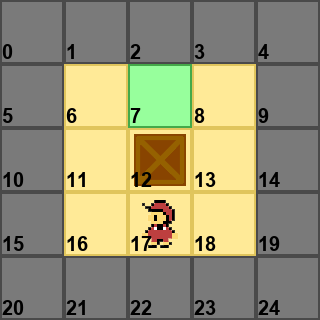
\includegraphics[width=4.5cm]{images/sokoban_simple.png}
    \caption{A simple Sokoban level with a position index on each tile.}
    \label{fig:sokoban_simple}
\end{figure}

\subsection{Non-deterministic transitions}
The probabilistic model is a Markov decision process (MDP). This type of model allows for both probabilistic and non-deterministic transitions. The moves in the model description are specified in such a way that they will be chosen non-deterministically. The moves can be in any direction, as long as the puzzle's layout allows for this. If the player is positioned at a tile $T$, they can walk to any adjacent tile $T'$, given that this tile is not a wall nor contains a box. If $T'$ does contain a box, the player will have to push the box forwards to the adjacent tile $T''$. This is only possible if $T''$ is not a wall nor contains a box. This means that for any combination of ($T$, $T'$), a walk transition exists, while a push transition between ($T$, $T'$) only exists if $T''$ is not a wall.

From position 12 in \autoref{fig:sokoban_simple}, only walk transitions exist, as the push condition cannot be satisfied. The transitions look as follows:
\lstinputlisting[language = PRISM]{code/walk_transitions.prism}
From all other reachable positions, the player can always push in one direction. Since the existence of a push transition into a direction also implies the existence of a walk transition into that same direction, the two moves are modelled as a single transition. This transition looks as follows from position 17:
\lstinputlisting[language=PRISM]{code/push_transition.prism}
The other two transitions, left and right, are again walk-only transitions. There is no down transition, as there is a wall at position 22.

Using these two types of transitions, a model checker can determine the shortest solution to this non-deterministic model.

\subsection{Probabilistic mistakes} 
Stochastic behaviour is added to the transitions, which forces the model checker to choose a suboptimal move with a predetermined probability. In this case, a suboptimal move is one that in most cases will increase the number of steps taken to solve the level. This behaviour is added by modifying the transitions so that with a probability of $\mu$, the player makes the optimal move. The remaining probability, $1 - \mu$, is divided into equal parts depending on the possible amount of alternative moves the player can make from that position. If the player cannot make the specified alternative move due to the current state of the board (for example because there are boxes in the way), the player does not move to prevent the model from deadlocking due to an invalid move.

The probabilistic up transition from position 12 in \autoref{fig:sokoban_simple} is modelled as follows:
\lstinputlisting[language=PRISM]{code/probabilistic_transition.prism}
From position 12, there are four possible walk moves: up, down, left, and right. The primary move, up in the example above, is chosen with a probability of $\mu$. The three alternative moves are chosen with a probability of $\frac{1 - \mu}{3}$. As only walk moves are permitted from this position, it is possible that a move cannot be executed because of a box being in the way. As mentioned above, the model must not deadlock due to invalid moves, thus the alternative moves are modelled using a ternary statement so that they are only executed if they are valid moves.

The concept remains the same if push moves are also permitted, however, due to the need to check and reassign more variables, these are more complex. The assignments for the walk/push move from position 12 to position 7 in \autoref{fig:sokoban_simple} are modelled as follows; for the sake of brevity, the guards and other irrelevant assignments are left out:
\lstinputlisting[language=PRISM]{code/probabilistic_push_transition.prism}

The probabilistic transitions have a significant consequence on the solvability of the levels. The model now forces the model checker to make a suboptimal move with the probability of $\mu$. While invalid moves will not be executed, it is now possible to make the level unsolvable by pushing a box into a position from which it can no longer be moved.

\subsection{Rewards}
\label{sec:rewards}
PRISM, Modest and Storm all support MDPs with transition rewards. This means that a certain cost can be attached to a transition, which can be used to calculate the total amount of moves taken to reach the required state. However, if the probability of reaching this state is less than 1, the rewards converge to infinity. Support for conditional reward properties for MDPs is missing in all three model checkers, meaning with the model described above, rewards cannot be used due to the fact that a mistake could make the level unsolvable. However, to still be able to calculate the expected amount of moves required to solve the level, the generation tool can also output models where a mistake can only be a walk move, not a push move. This means a level will never be unsolvable, as a walk move can always be undone; thus, the rewards work as expected.

\subsection{Generation}
The model generation tool generates probabilistic models as described above from Sokoban levels supplied by the user as .sok files. The generated models are described by the PRISM language and the JANI specification so that a wide range of probabilistic model checkers can be targeted. The generated models contain an undefined constant, $\mu$, that defines the probability that the player makes the best move. A high-level overview of the workings of the tool is as follows:
\begin{enumerate}
    \item Parse a .sok file into an intermediate representation that better suits the generation process.
    \item Run a depth-first search starting from the player's position to find all reachable tiles.
    \item Generate the variables used to encode the player and box positions.
    \item Iterate over all possible moves for each reachable tile and generate the transitions between the states.
\end{enumerate}
